\newpage

\section{Design}
I vores design har vi vægtet at hver class vi implementere har ét ansvar. Det vil sige at det ikke nødvendigvis er den class som indeholder informationen som bearbejder den. At følge dette princip har den svaghed at kommunikationskæden vil blive længere end den behøver hvilket ultimativt vil lede til at vores program vil køre langsommere. Tilgengæld vil vores kodebase være nemmere at maintain da det vil blive tydeligt hvor hvilken opgave bliver udført og det vil derfor også blive nemmere at identificere hvor bugs opstår. Vi har også fulgt princip om at hver klasse selv udfører sit arbejde og vi har derfor ikke klasser som er afhængige af andre klassers metoder, men vi har klasser som er afhængige af andre klasser.\\
Vi kan bekræfte det ovenstående ud fra vores traceability matrix som mapper hvert af vores koncepter med use cases. Vores traceability matrix indikerer at hver af vores klasser kun har ét ansvar idet at få koncepter matcher flere use cases. Mængden af klasser kan være en indikation på at kommunikationskæden er lang, mens det at der ikke er mange koncepter som mapper til mere end en use case fortæller os at arbejdsbyrden er jævnt fordelt.\\

\begin{table}[h!]
\centering
\label{my-label}
\begin{tabular}{|l|l|l|l|l|l|l|l|l|l|}
\hline
               & LL & FR & LCl & LCr & EC & LK & GameState & StateMachine & SpaceBus \\\hline

Load Levels   &          x           &            &       &      &              &       &       &       &      \\\hline
Læs filer    &         &              x          &       &      &              &       &       &       &       \\\hline
Level class        &         &             &             x    &      &              &      &       &          &     \\\hline
Lav et level  &         &             &            &       x&                   &       &       &       &       \\\hline
Lav en entity &         &             &            &       &     x &                      &       &       &     \\\hline
Hold Levels   &         &             &            &       &      &x            &            &       & \\\hline
Pause Game &         &             &            &       &      &                      &x       &       &     \\\hline
Menu &         &             &            &       &      &                      &x       &       &     \\\hline
Tab spil &         &             &            &       &      &                      &x       &       &     \\\hline
Kør spil &         &             &            &       &      &                      &x       &       &     \\\hline
Skift state &         &             &            &       &      &                      &       &x       &     \\\hline
Inputs &         &             &            &       &      &                      & x           & x   & x  \\\hline
\end{tabular}
\end{table}

Ud fra vores sequence diagram, som ses på figur \ref{seqDig}, kan det ses at vores design arbejder af flere omgange. LevelLoader beder FileReader om at læse en levelfil hvorefter at FileReader benytter informationerne fra levelfilen til kalde konstruktoren i Level for at lave et nyt level objekt som bliver givet tilbage til LevelLoader. I LevelLoader hentes der en instans af LevelsKeeper som bruges til at gemme level objektet. Dette loop bliver gentaget for alle de levelfiler som er specificeret i LevelLoader hvilket udgør den første del af vores design. LevelLoader bliver brugt ude i Program hvilket sørger for at alle levels i spillet er loadet inden brugeren får givet nogen form for kontrol. Dette vil kunne give problemer med hastigheden af opstart af spillet hvis der skal loades en meget stor mængde af levels, mens at det vil sikre en hurtig transition mellem levels. Da vi ikke forventer der skal loades store mængder af levels, så vil vi placere en lille ventetid i opstarten af programmet og dermed opnå et hurtigt skift mellem levels. \\
Dernæst bliver Game instantiatet hvilket resulterer i instantiationen af SpaceBus, StateMachine og MainMenu.\\
Herefter køres GameLoop i Game hvilket begynder spillet. Når der trykkes 'New Game' fra menuen så skifter StateMachine den aktive state til GameRunning ved hjælp af StateTransformer. Når GameRunning bliver kørt bedes LevelCreator om en liste af EntityContainers for de blokke som skal udgøre det level som skal tegnes. LevelCreator indeholder også en instans af LevelsKeeper som nu benyttes til at hente et specifikt level som er blevet gemt. LevelCreator benytter oplysningerne i det hentede level objekt til at bede EntityCreator om at lave en ny entity som skal udgøre en blok i et level. LevelCreator gemmer denne entity i en EntityContainer, og når alle blokke er blevet bygget returneres listen af EntityContainere og GameRunning kan derefter render dem.\\
Da alle vores GameStates er meget ens, så er de samlet under det samme interface. Dette bevirker at StateMachine skal holde en instans af en 'IGameState'. Vores StateMachine er indført ved principperne om en statemachine, men da vi ikke har lørt om dette design pattern kan vi kun beskrive det som en form for implementation af et Mediator pattern som sørger for kommunikationen mellem vores game states.\\

\subsection{Design principper}
Som tidligere beskrevet har vi lagt stor vægt på Single Responsibility Princippet og vi ser at dette princip i høj grad bliver opfyldt. Hver klasse har en enkelt opgave som den selv løser. Det kan diskuteres om StateMachine og StateTransformer bør være én klasse, men vi har valgt at se StateMachines ansvar som den klasse der skifter states og StateTransformers som værende at oversætte events. Vi har således to ansvar til to klasser men de arbejder sammen om at udføre et fælles mål.\\
Ud fra vores traceablity matrix ser vi at flere af vores koncepter håndterer input. Dette er muligvis en smule misledende idet at alle koncepterne får hjælp af SpaceBus til dette. Da SpaceBus fungerer som en observer så er det ikke underligt at de klasser som benytter SpaceBus alle vil håndtere inputs.\\

Ønsker vi at udvide med flere GameStates så kan det ikke lade sig gøre uden at skulle udvide både StateTransformer og StateMachine. Dette betyder at vi ikke følger Open/closed pricippet og det er altså ikke ligetil at skulle udvide vores spil. Dog ser vi at princippet kan følges i forhold til LevelCreator og EntityCreator idet at vi kan skabe en ny type af blokke til vores level ved kun at ændre LevelCreator.\\

Selvom Liskov Substitution pricippet ligger Open/closed princippet nært, så ser vi alligevel at dette princip er fulgt. Idet vores GameStates er samlet under samme interface, så kan vi nemlig nemt skifte states. Selvom det er besværligt at indføre nye GameStates til spillet, så er det altså ligetil at skifte GameState.\\

Desværre ser vi at IGameState interfacet er for bredt, idet flere af vores states ikke har en implementation for flere af de definerede metoder. Vi følger derfor ikke Interface segregation princippet. Da IGameState er defineret i DIKUArcade har vi valgt ikke at ændre interfacet selvom det ville være nemt og hurtigt derved at følge princippet.\\

\begin{figure}[h!]
  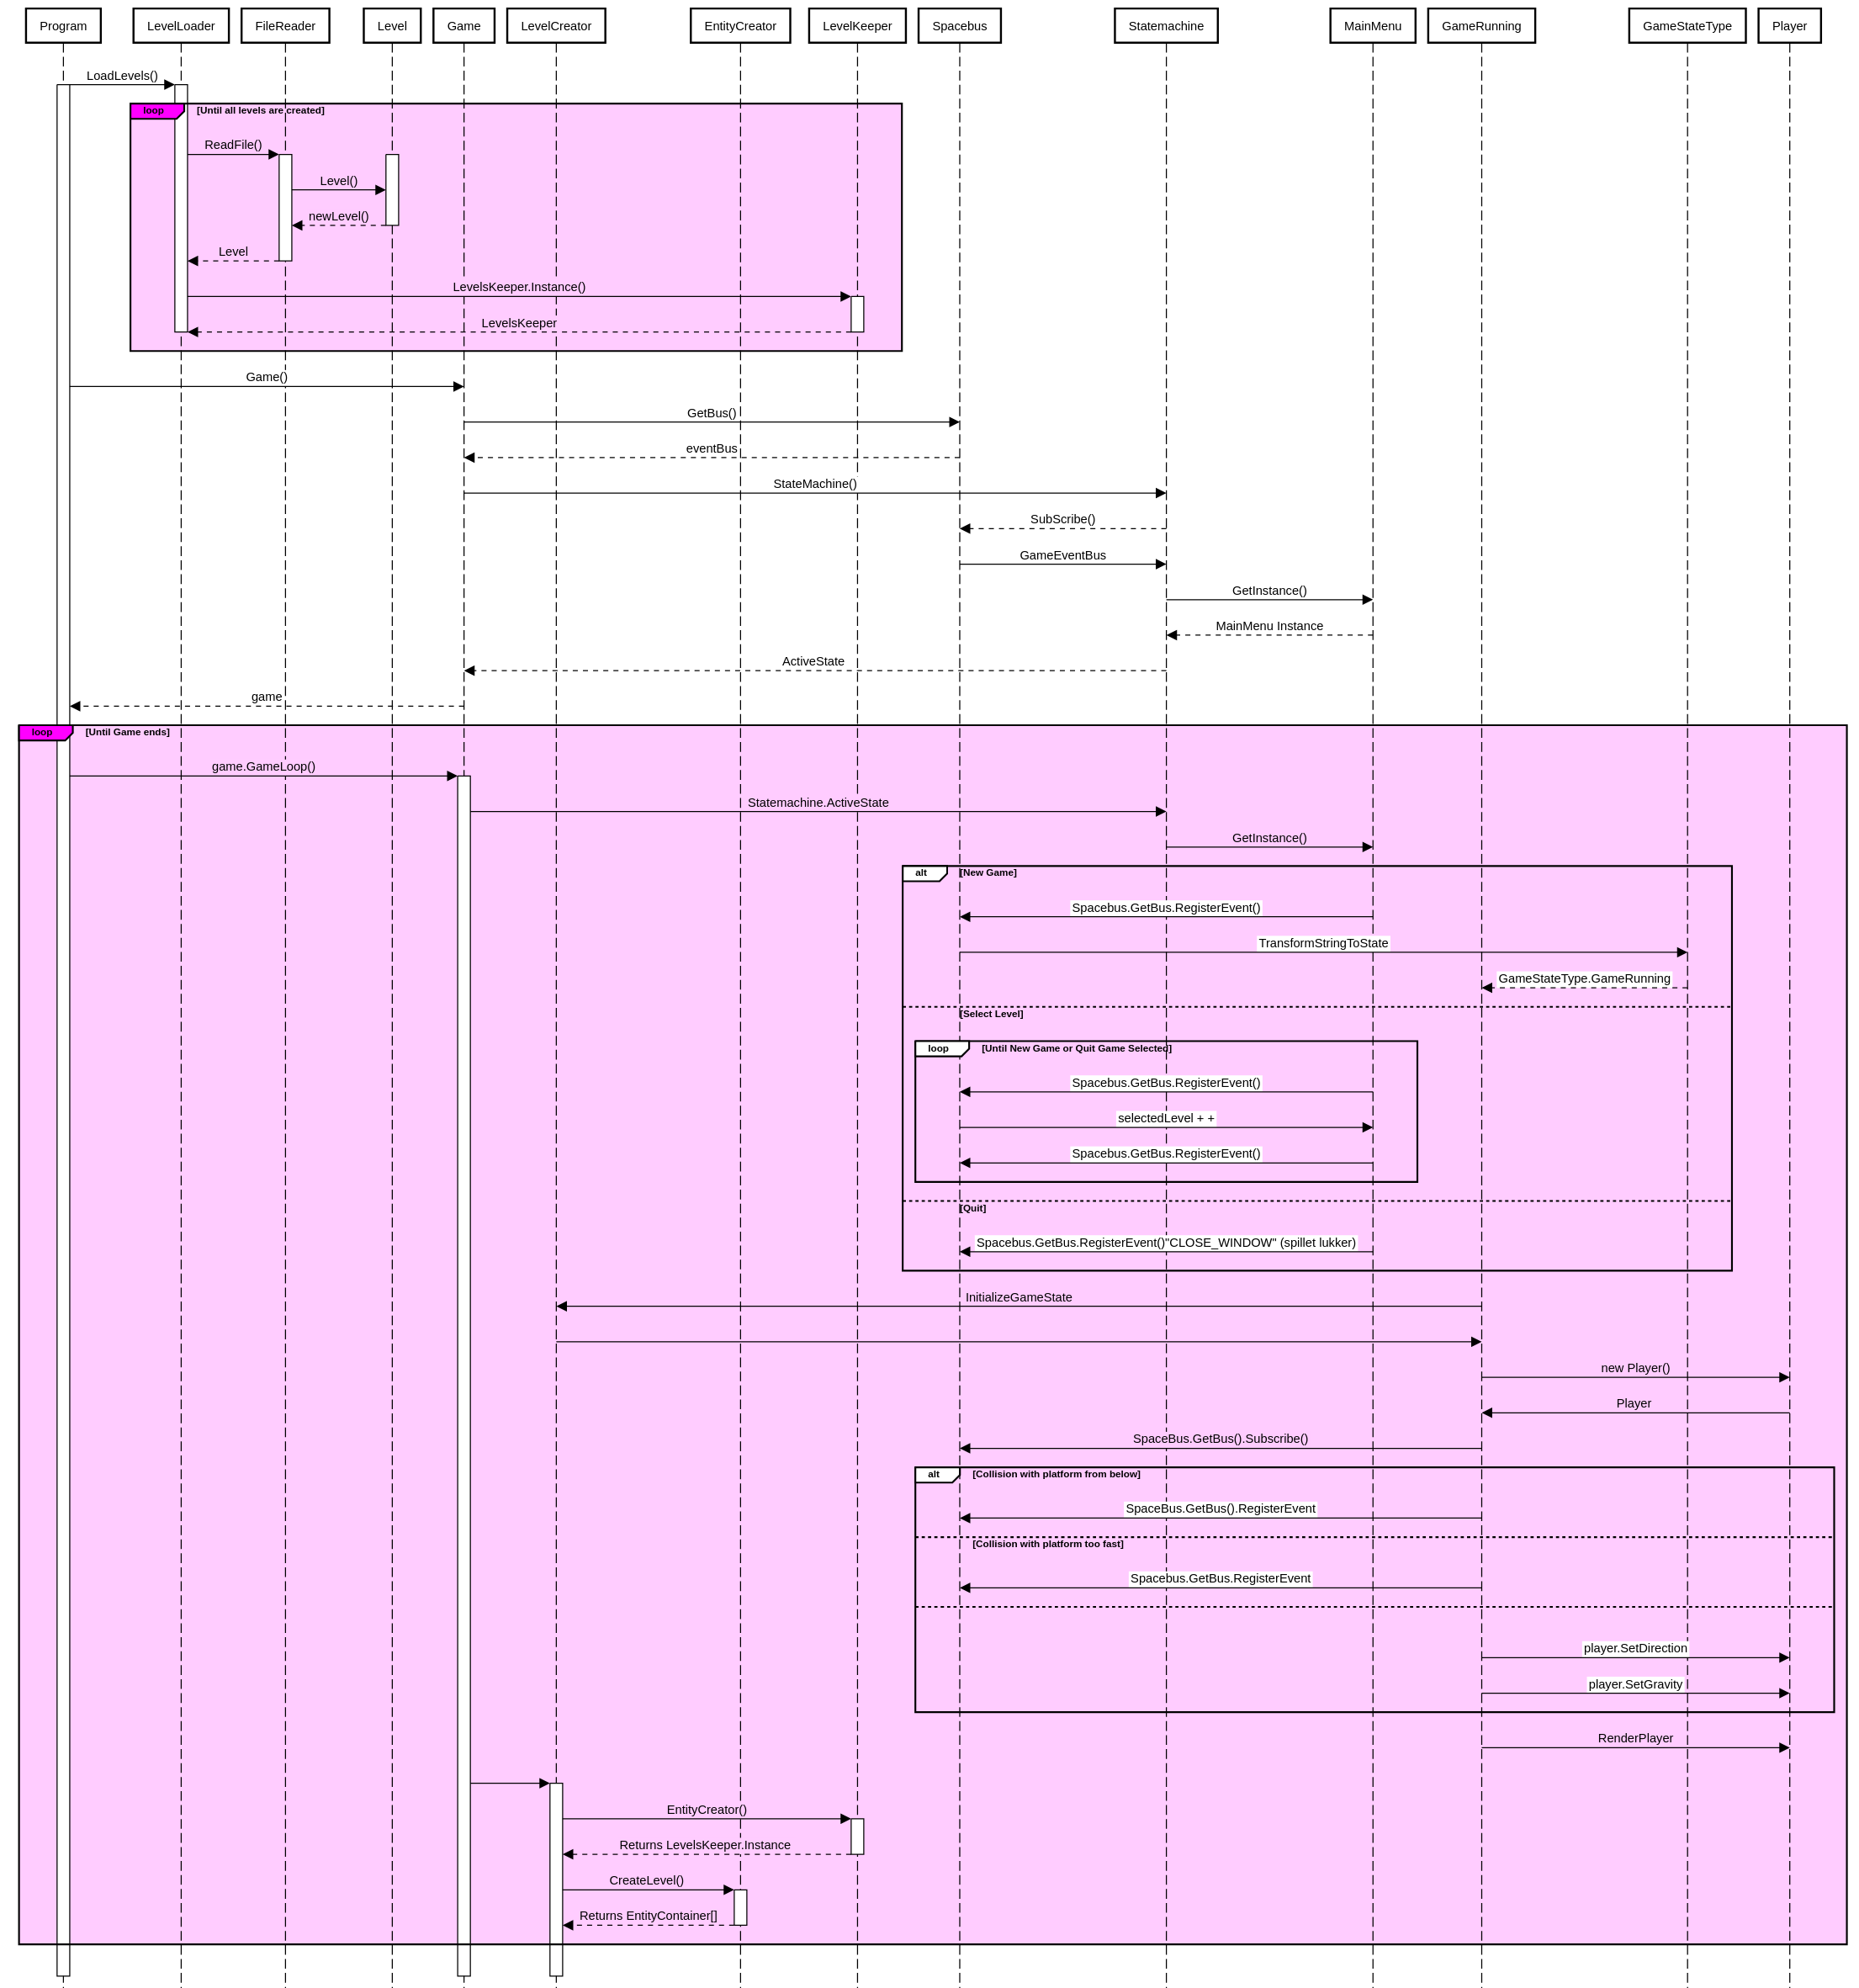
\includegraphics[width=\linewidth]{latex/Images/SequenceDiagram.png}
  \caption{Sequence diagram}
  \label{seqDig}
\end{figure}
